% Ubah judul dan label berikut sesuai dengan yang diinginkan.
\section{INTRODUCTION}
\label{sec:pendahuluan}

% Ubah paragraf-paragraf pada bagian ini sesuai dengan yang diinginkan.

Social media is a medium to socialize with each other and is done online which allows humans to interact with each other without being limited by space and time \cite{media_sosial}. Social media removes human boundaries to socialize, space and time limits, with this social media humans are allowed to communicate with each other wherever they are and at any time, no matter how far apart they are, and no matter day or night. Social media has a huge impact on our lives today. Someone who is originally "small" can instantly become big with social media, and vice versa "big" people in a second can become "small" with social media.

But along with the positive impact, social media also has a negative impact in the form of rampant Negative Emotion Tweet on social media. This is very worrying because social media in today's era can be said to be included as a primary human need. In addition, from year to year or even day to day, the amount of Negative Emotion Tweet on social media shows absolutely no signs of disappearing or being resolved. One of the causes of this is the rise of social media users who just follow along, either spreading or making the same upload without knowing the original intent/message/type of an upload because it is being discussed\cite{ujaran_kebencian}.


Based on a survey conducted by the company \textit{Microsoft} entitled \textbf{Digital Civility Index}, which is a survey on the behavior of citizens who have been surveyed in using \textit{Platform} Technology, Indonesia has a relatively low score compared to other Asean countries in behaving on Social Media with a ranking of 29 out of 32 countries. This survey was conducted annually in the last five years and had 16,000 respondents in 32 countries. Of course this is very bad for Indonesia because the survey reflects the behavior of its citizens in using social media\cite{dci}.

The impact given by the rise of Negative Emotion Tweet will not only be felt by each individual, but the impact of this can also be felt by the international community. The existence of Negative Emotion Tweet directed at citizens of other countries can cause conflict and disrupt international relations between the two countries. Based on Mai Elsherief's research, the majority of Negative Emotion Tweet spreaders on social media use pseudonyms for their accounts in order to avoid knowing their real identities. In addition they generally target accounts that have a large number of followers or accounts that have a high level of activity\cite{dampak_kebencian}.

There have been several government efforts to overcome this problem by taking two approaches, namely preventive and repressive. The preventive approach can start from handling content related to Negative Emotion Tweet, while the repressive approach is more towards law enforcement related to legal efforts or processes.\cite{kominfo}. However, this step has not been effective because until now there are still many Negative Emotion Tweet on social media. 

\textit{Neural Networks} is a branch of machine learning that uses \textit{neurons} like the structure of the human brain to process data and generate output. One of the relatively new \textit{neural network} methods is \textit{Bi-directional Encoder Representations from Transformers} or BERT for short. BERT is a method used to get context in an entered text, this makes BERT very suitable for performing tasks based on NLP (\textit{Natural Language Processing}). Even so, in Indonesia there are still not many implementations of BERT itself.

\begin{figure}[h]
    \begin{center}
        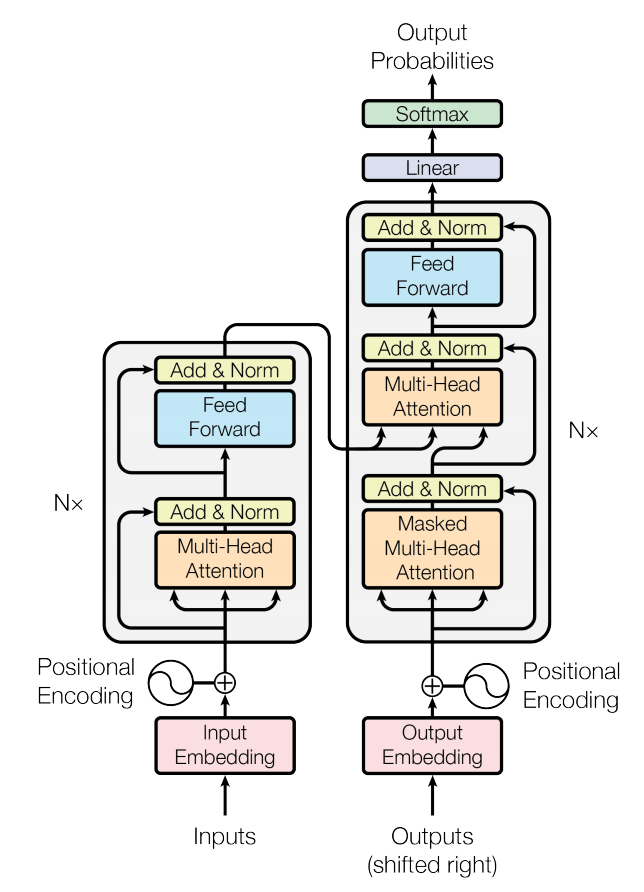
\includegraphics[width= 0.9\linewidth]{template-paper-ieee-main/gambar/04_transformer.png}
        \caption{Transformers Architecture That will be use in the Research}
        \label{fig: transformers}
    \end{center}
\end{figure}

\begin{figure}[h]
    \begin{center}
        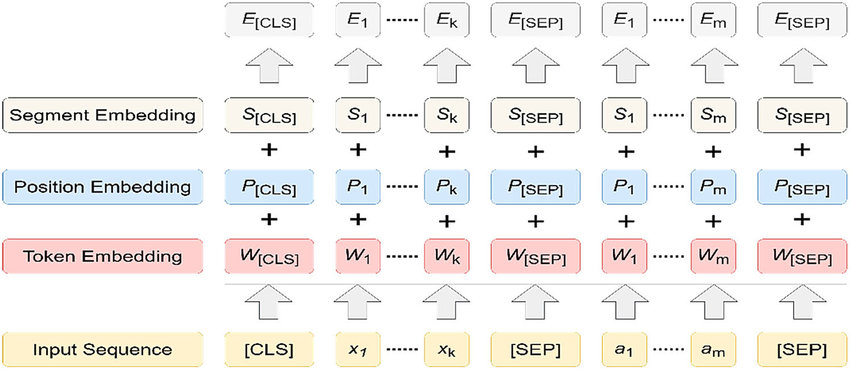
\includegraphics[width= 0.9\linewidth]{template-paper-ieee-main/gambar/05_berttoken.png}
        \caption{BERT Architecture That will be use in the Research}
        \label{fig: bert}
    \end{center}
\end{figure}



\section{PREVIOUS RESEARCH}
\label{sec:penelitianterdahulu}

In the research entitled \textit{Emotion Detection and Analysis on Social Media}, the problem of detecting, classifying and quantifying text emotions in any form is discussed. This study uses English text collected from social media such as \textit{Twitter}, which can provide useful information in various ways, especially opinion mining. Social media like \textit{Twitter} and \textit{Facebook} are full of emotions, feelings and opinions of people all over the world. However, analyzing and classifying text on the basis of emotion is a big challenge and can be considered as an advanced form of \textit{Sentiment Analysis}. This \textit{Paper} proposes a method for classifying text into six different Emotion-Categories: Happiness, Sadness, Fear, Anger, Shock, and Disgust. The model used is, the author uses two different approaches and combines them to effectively extract these emotions from the text. The first approach is based on \textit{Natural Language Processing}, and uses some textual features such as \textit{Emoticons}, word degrees and negation, Part Of Speech and other grammatical analysis. The second approach is based on the \textit{Machine Learning} classification algorithm. We have also successfully devised a method to automate the creation of the \textit{Training Set} itself, eliminating the need for manual annotation of large data sets. In addition, this research has succeeded in creating \textit{Bag of Words} emotional words, along with their emotional intensity. On testing, it appears that this research model provides significant accuracy in classifying \textit{tweet} taken from \textit{Twitter}.

A similar study entitled \textit{Emotion Detection Framework for Twitter Data Using Supervised Classifiers} has more or less the same goal. The research has the objective of emotion detection which involves text analysis. Humans show universal consistency in identifying emotions but show a great deal of variation between individuals in their abilities. This study has detected emotions for \textit{Twitter} messages because they provide an ensemble of human emotions. This research has used machine learning algorithms or \textit{Machine Learning} namely \textit{Naive Bayes (NB)} and \textit{k-nearest neighbor (KNN)} algorithms to detect the emotion of \textit{Twitter} messages and then classify messages \textit{Twitter} into four emotional categories. We also made a comparative study of two supervised machine learning algorithms; \textit{Classifier} NB performs well when compared to \textit{Classfier} KNN .

Another research entitled \textit{Emotion Recognition by Textual Tweets Classification Using Voting Classifier (LR-SGD)} has a background problem, namely the proliferation of user-generated content on social media has made opinion mining a difficult task. As a \textit{microblogging} platform, \textit{Twitter} is used to gather views on products, trends and politics. Sentiment analysis is a technique used to analyze different people's attitudes, emotions and opinions towards anything, and can be done on \textit{tweet} to analyze public opinion about news, policies, social movements and personalities. By using the \textit{Machine Learning} model, opinion mining can be done without reading \textit{tweet} manually. Their results can help governments and businesses launch policies, products and events. The \textit{Seven Machine Learning} model is implemented for emotion recognition by classifying \textit{tweet} as happy or unhappy. With an in-depth comparative performance analysis, it was observed that the proposed voting classifier \textit{(LR-SGD)} with \textit{TF-IDF} yielded the most optimal results with an accuracy of 79\% and an F1 score of 81\%. To further validate the stability of the proposed approach on two more datasets, one binary dataset and another \textit{multiclass} dataset and achieve robust results.

Of the three studies, the \textit{Supervised Learning} and \textit{Natural Language Processing} methods were successful in classifying the \textit{Emotion} type in \textit{Twitter} Text. textbf{BERT} to apply to text detection \textit{Emotion} \textit{TWitter} in Indonesian. Based on the data and information presented in the previous section, it is necessary to conduct research to classify the types of \textit{Emotion}
\textit{Twitter} Indonesia. In the future, the system can be developed into something useful, such as preventing Negative Emotion Tweet on social media.